O padrão CMSIS (\emph{Cortex Microcontroller Software Standard}) é um \emph{framework} para aplicações embarcadas criado pela própria \href{http://infocenter.arm.com/help/index.jsp}{ARM Limited}, que define um padrão de API de acesso ao hardware para processadores da linha Cortex-M, de modo a simplificar o desenvolvimento e manutenção dos códigos-fonte.

A implementação do CMSIS geralmente é fornecida pelo fabricante do microcontrolador no qual se está utilizando, desde que este possua um processador Cortex-M. No entanto, se o fabricante não fornecer a implementação do CMSIS é possível implementá-lo baseando-se nos exemplos e usando os \emph{templates} fornecido no site da \href{http://www.arm.com/products/processors/cortex-m/cortex-microcontroller-software-interface-standard.php}{ARM Limited}.

Segundo YIU\cite{ARMGUIDE}, CMSIS é um projeto em constate evolução, sendo que o primeiro componente desta biblioteca, o  CMSIS-CORE, visava apenas estabelecer a consistência das bibliotecas de \emph{drivers}. Desde então a biblioteca CMSIS tem somado cada vez mais componentes em sua biblioteca. Atualmente há 5 componentes, sendo: 

\begin{itemize}
	\item \textbf{CMSIS-CORE:} Conjunto de APIs necessárias para acessar os recursos do processador Cortex-M e dos demais periféricos, independente do microcontrolador ou conjunto de ferramentas utilizadas.
	
	\item \textbf{CMSIS-DSP:} Biblioteca de rotinas que possibilita criar facilmente diversas aplicações DSP no Cortex-M, suportando uma grande variedade de operações matemáticas, desde operações básicas de matrizes até calculo de FFT e filtros digitais. 
	
	\item \textbf{CMSIS-RTOS:} API de interface para RTOS (\emph{Real Time Operating System}). Isto permite desenvolver códigos para múltiplas plataformas de sistemas operacionais embarcados.
	
	\item \textbf{CMSIS-DAP:} Arquivo de referência, ou \emph{firmware}, necessário para criar um adaptador de interface de depuração. Isso permite que os adaptadores de depuração de baixo custo que utilizam vários \emph{toolchains} possam ser desenvolvidos.
	
	\item \textbf{CMSIS-SVD:} É um arquivo no formato XML que descreve o microcontrolador e todos os periféricos presentes.
\end{itemize}

\section{CMSIS-CORE}

Dentro da biblioteca CMSIS, no componente CMSIS-CORE, há diversos pacotes de \emph{drivers} para diferentes dispositivos. Alguns destes pacotes são criados pela \href{http://infocenter.arm.com/help/index.jsp}{ARM Limited}, outros são criados pelos próprios fabricantes de microcontroladores.  Porém em um sentido geral CMSIS-CORE é padronizado com um conjunto de múltiplas camadas, sendo estas:

\begin{itemize}
	\item \textbf{Camada de Acesso ao Processador:} Aqui são feitas as definições de endereços, funções auxiliares para acessar os registradores e os periféricos do processador.
	
	\item \textbf{Camada de Acesso a Dispositivos Periféricos:} Nesta camada é definido os endereços dos registradores dos periféricos, bem como a implementação básica do sistema, incluindo o vetor de interrupção.
	
	\item \textbf{Camada de Funções de Acesso aos Periféricos:} É a camada que contem os \emph{drivers} para acesso de periféricos fornecido pelo fabricante do microcontrolador. É possível escolher entre usar o código do fabricante ou programar os periféricos manualmente. 
\end{itemize}

A Figura \ref{fig:CMSIS-CORE} apresenta um diagrama base que representa os níveis da estrutura presente no CMSIS-CORE. Entender como os diferentes níveis da estrutura se relacionam é essencial para  utilizar a biblioteca CMSIS.

\begin{figure}[!h]
	\centering
	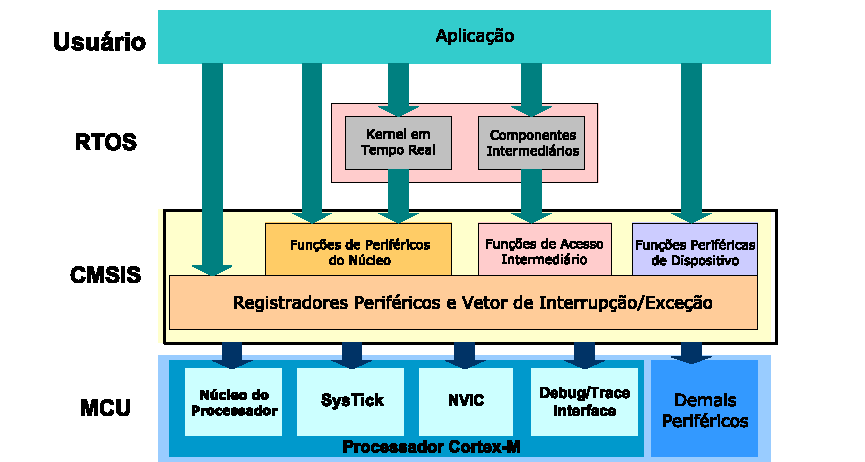
\includegraphics[width=1\textwidth] {figuras/CMSIS-CoreStructure.pdf}
	\caption{Estrutura do CMSIS-CORE}
	\label{fig:CMSIS-CORE}
\end{figure}


\section{Incluindo o CMSIS ao Projeto}

Para incluir o CMSIS a um projeto e utilizar tanto  o CMSIS-CORE quanto os demais componentes desta biblioteca é necessário seguir os seguintes passos: 

\begin{enumerate}
	\item Adicionar os aquivos fonte no projeto, que incluem:
	\begin{itemize}
		\item \textbf{startup\_<device>.c:}  Sendo este o código básico de inicialização. Incluindo a rotina de \emph{reset}, a configuração do \emph{Stack-Pointer} e a tabela de vetores de interrupção. Pode estar implementado tanto em linguagem C como em Assembly.
		\item \textbf{system\_<device>.c:} Este arquivo possui as rotinas genéricas de configuração, sendo portanto responsável pela inicialização dos dispositivos específicos do microcontrolador usado.
		\item  \textbf{Fontes adicionais:} São arquivos fonte adicionais fornecidos pelo fabricante do microcontrolador. Não possuem uma sintaxe padrão e sendo que sua inclusão no projeto é opcional. 
		\item \textbf{core\_c<core>.c:} Este arquivo é necessário apenas para versões de CMSIS inferiores a 2.0. De cordo com o processador utilizado seleciona-se o arquivo correspondente, para que assim seja possível  acessar algumas das funções dos  registadores do processador.
	\end{itemize}
	
	\item Adicionar os arquivos de cabeçalho, que incluem:
	\begin{itemize}
		\item \textbf{<device>.h:} Arquivo de cabeçalho específico do microcontrolador, que define os registradores dos periféricos e as definições do vetor de interrupções.
		\item \textbf{system\_<device>.h:} Arquivo de cabeçalho específico para as rotinas genéricas de configuração. É essencial para o funcionamento do arquivo \emph{system\_<device>.c}.
		\item \textbf{core\_c<core>.h:} Cabeçalho específico referente ao processador utilizado.
		\item  \textbf{Cabeçalhos Adicionais:} Cabeçalhos fornecidos pelo fabricante do microcontrolador. Estes cabeçalhos estão relacionados ao acesso de periféricos, porém a inclusão destes cabeçalhos é opcional.
	\end{itemize}
\end{enumerate}

\section{Com o Code Composer Studio}

Ao utilizar uma versão igual ou superior à 6.1.3 do Code Composer, após a criação do projeto, já serão incluídos os arquivos referentes à CMSIS necessários para a utilização no MSP432. Não sendo necessária nenhuma alteração.

Se for utilizada uma versão antiga, há uma atualização disponível que pode ser acessada diretamente da IDE em uma máquina com acesso à Internet. Os passos podem ser seguidos no \emph{link} oficial da Texas Instruments (\href{http://processors.wiki.ti.com/index.php/MSP432_CMSIS_Update}{MSP432 CMSIS Update}).
